%!TEX root = ./template-skripsi.tex
%-------------------------------------------------------------------------------
%                            BAB III
%               			PEMBAHASAN
%-------------------------------------------------------------------------------

\chapter{METODOLOGI PENELITIAN}

Melalui penelitian yang dilakukan oleh penulis, akan menghasilkan produk tertentu. Penelitian yang dilakukan oleh penulis juga termasuk dalam jenis penelitian dan pengembangan. Berikut adalah tahapan-tahapan penelitian yang penulis lakukan dalam perancangan sebuah aplikasi:

\begin{figure}[H]
	\centering
	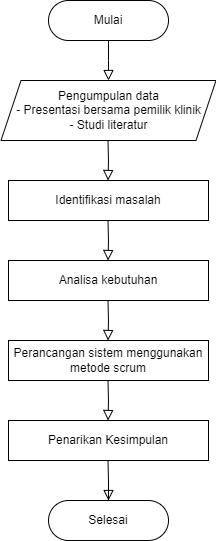
\includegraphics[width=4cm]{gambar/tahapan penelitian fix.png}
	\caption{Tahapan penelitian} 
	\label{Gambar:usecaseadminjurnalpertama}
\end{figure}

\section{Pengumpulan Data}

Peneliti mengambil data dari presentasi bersama dengan pemilik klinik \emph{moist care} dan klien dari penelitian ini yaitu ibu Irma Puspita Arisanti. Untuk dokumentasi foto pada saat presentasi dapat dilihat pada Lampiran A. Peneliti juga melakukan studi literatur dengan membaca jurnal-jurnal yang berkaitan dengan topik penelitian serupa. 

\section{Analisa Kebutuhan}
Berikut merupakan perangkat keras dan perangkat lunak yang penulis butuhkan dalam merancang sistem informasi keperawatan luka:

Perangkat keras berupa:
\begin{enumerate}
	
\item Laptop dengan spesifikasi Processor Intel Core i5 generasi ke-3 dan RAM 12 GB.
	
\end{enumerate}

Perangkat lunak berupa:
\begin{enumerate}
\item Windows 10 \emph{Operating System}.

\item Figma sebagai alat untuk mendesain tampilan UI/UX.

\item \emph{Visual Studio Code} untuk pembuatan sistem informasi keperawatan luka.

\item \emph{Python} sebagai bahasa pemrograman yang peneliti gunakan.

\item \emph{Flask} sebagai web framework yang akan digunakan.

\item MongoDB sebagai basis data
\end{enumerate}

\section{Perancangan Sistem Menggunakan \emph{Scrum}}

\emph{Website} aplikasi yang dibuat dalam penelitian ini dikembangkan dengan menggunakan metode \emph{scrum}. Penjelasan rinci tentang metode \emph{scrum} akan disajikan pada sub bab di bawah ini.

\subsection{\emph{Product Backlog}}

Tahap \emph{Product backlog} ini berfungsi untuk menterjemahkan seluruh fitur yang akan diimplementasikan pada aplikasi. Rincian \emph{Product Backlog} yang akan diimplementasikan pada \emph{website} aplikasi dapat dilihat pada tabel di bawah ini.

\begin{table}[H]
	\centering
	\caption{\emph{Product Backlog}}
	\label{tabel_input}
	\begin{tabular}{|c|l|c|c|}
		\hline
		\textbf{No} & \textbf{\emph{User Story}} & \textbf{\emph{Priority}} & \textbf{\emph{Sprint} No.} \\
		\hline
		
		1 & 
		Pembuatan akun pasien & \emph{High}
		& 1 \& 2 \\
		\hline
		
		2 & 
		Dashboard klinik  & \emph{High}
		& 1 \& 2 \\
		\hline
		
		3 & 
		Pemeriksaan kesehatan & \emph{High}
		& 1 \& 3 \\
		\hline
		
		4 & 
		Proses pengobatan luka & \emph{High}
		& 1 \& 3 \\
		\hline
		
		5 & 
		Pendaftaran pasien berobat & \emph{High}
		& 1 \& 3 \\
		\hline
		
		6 & 
		Pengelolaan antrian & \emph{High}
		& 1 \& 4 \\
		\hline
		
		7 & 
		Administrasi keuangan  & \emph{High}
		& 1 \& 4 \\
		\hline
		
	\end{tabular}
\end{table}

\emph{Product backlog} yang dibuat memiliki 4 kolom yang di antaranya adalah sebagai berikut:

\begin{enumerate}
	\item \emph{User Story}
	
	Kolom \emph{user story} berisi fitur-fitur yang akan dibuat pada aplikasi.
	
	\item \emph{Priority}
	
	Kolom \emph{priority} berisi tingkat priortas dari \emph{user story}, dimana prioritas \emph{high} merupakan fitur yang mempunyai peran penting pada penelitian ini.
	
	\item \emph{Sprint} No.
	
	Kolom \emph{sprint} no. berisi informasi tentang urutan pengerjaan fitur \emph{sprint} tersebut akan dibuat.
\end{enumerate}

\subsection{\emph{Sprint Backlog}}
Sebelum \emph{sprint} dimulai dilakukan \emph{sprint backlog}, \emph{sprint backlog} berisikan daftar pekerjaan yang keputusannya diambil dari \emph{product backlog}. Dengan adanya \emph{sprint backlog} semua anggota tim bisa melihat perkembangan dari setiap pekerjaan. Pada penelitian peneliti menggunakan tiga status perkembangan yaitu harus dikerjakan, sedang dikerjakan, selesai, next \emph{sprint} dan tidak selesais.

\subsection{\emph{Sprint}}
Setelah perencanaan \emph{sprint backlog} sudah dibuat, maka pengerjaan \emph{sprint} sudah bisa dimulai dan mengikuti jadwal pengerjaan yang telah disepakati bersama tim. Interval \emph{sprint} yang digunakan adalah dua minggu.

\subsection{\emph{Deploy}}
Setelah semua pekerjaan \emph{sprint} yang telah direncanakan pada sprint backlog selesai maka aplikasi akan di \emph{deploy}.

\begin{comment}
	
	Mockup administrasi keuangan
	Penjelasan UI/UX bab 2 revisi banyak
	API route setiap fitur
	
	
	menjelaskan sistem utuh yang dibuat salsa
	membuat product backlog yang berisi 3 sprint, rancangan ui dan data base
	
	sprint 1 berisi
	1. database diagram
	2. produk backlog
	3. rancangan ui/ux
	yang dibagi per iterasi
	
	implementasi sprint 1
	
	acc sps

\begin{table}[H]
	\centering
	\caption{\emph{Sprint}-2 \emph{Backlog}}
	\label{tabel_input}
	\begin{tabular}{|c|m{6 cm}|m{6 cm}|}
		\hline
		\textbf{No} & \textbf{\emph{User Story}} & \textbf{\emph{Task}}\\
		\hline
		
		1 & 
		Pembuatan akun pasien & 1.Pembuatan akun pasien.\\
		
		& 
		& 2.Menerima pendaftaran akun pasien baru\\
		\hline
		
		2 & 
		Pendaftaran pasien berobat & 1.Melakukan pendaftaran pasien yang berobat pada hari H.\\
		
		& 
		& 2.Mencari data pasien berdasarkan \emph{Medical} ID/Nomor BPJD/NIK.\\
		
		& 
		& 3.Sistem mampu mengeluarkan nomor antrean pengobatan secara \emph{real time}.\\
		\hline
		
	\end{tabular}
\end{table}

\begin{table}[H]
	\centering
	\caption{\emph{Sprint}-3 \emph{Backlog}}
	\label{tabel_input}
	\begin{tabular}{|c|m{5 cm}|m{6 cm}|m{1 cm}|}
		\hline
		\textbf{No} & \textbf{\emph{User Story}} & \textbf{\emph{Task}} & \textbf{\emph{Status}} \\
		\hline
		
		1 & 
		Pengelolaan antrean & 1.Menentukan kuota jumlah pelayanan pasien pada hari pelayanan
		& belum selesai \\
		
		& 
		& 2.Menentukan kuota pelayanan pasien \emph{online} pada hari pelayanan.
		& \\
		
		& 
		& 3.Menentukan kuota pelayanan pasien \emph{offline} pada hari pelayanan.
		& \\
		\hline
		
		2 & 
		Proses pengobatan & 1.Melihat hasil pengkajian luka dengan mencari berdasarkan NIK/Nama
		& belum selesai \\
		
		& 
		& 2.Melihat \emph{database} foto luka yang dikategorikan berdasarkan perawat
		& \\
		
		& 
		& 3.Inventarisasi komponen kesehatan yang masuk ke dalam klinik beserta harganya sebagai \emph{base cost}.
		& \\
		
		& 
		& 4.Menentukan tarif pengobatan diluar obat dan balutan(biaya layanan, dll).
		& \\
		\hline
		
	\end{tabular}
\end{table}

\begin{table}[H]
	\centering
	\caption{\emph{Sprint}-4 \emph{Backlog}}
	\label{tabel_input}
	\begin{tabular}{|c|m{5 cm}|m{6 cm}|m{1 cm}|}
		\hline
		\textbf{No} & \textbf{\emph{User Story}} & \textbf{\emph{Task}} & \textbf{\emph{Status}} \\
		\hline
		
		1 & 
		Administrasi keuangan & 1.Verifikasi dan validasi biaya tagihan
		& belum selesai \\
		\hline
		
		2 & 
		Dashboard klinik & 1.Melihat statistik kinerja perawat per bulan
		& belum selesai \\
		
		& 
		& 2.Melihat \emph{cost} dari inventarisasi yang tersedia dan aset yang masih berjalan.
		& \\
		
		& 
		& 3.Melihat besar \emph{cost} perawatan pasien.
		& \\
		
		& 
		& 4.Melihat \emph{income} masuk klinik
		& \\
		
		& 
		& 5. Melihat \emph{balance} keuangan dalam satu bulan
		& \\
		\hline
		
	\end{tabular}
\end{table}

\end{comment}